\documentclass[../rapport.tex]{subfiles}
\graphicspath{{\subfix{ressources/photos_diagrammes/app2/}}}

\usepackage[utf8]{inputenc}
\usepackage[french]{babel}
\usepackage{amsmath, amsfonts, amssymb, amsthm}

\begin{document}

\begin{figure}[h]
		\centering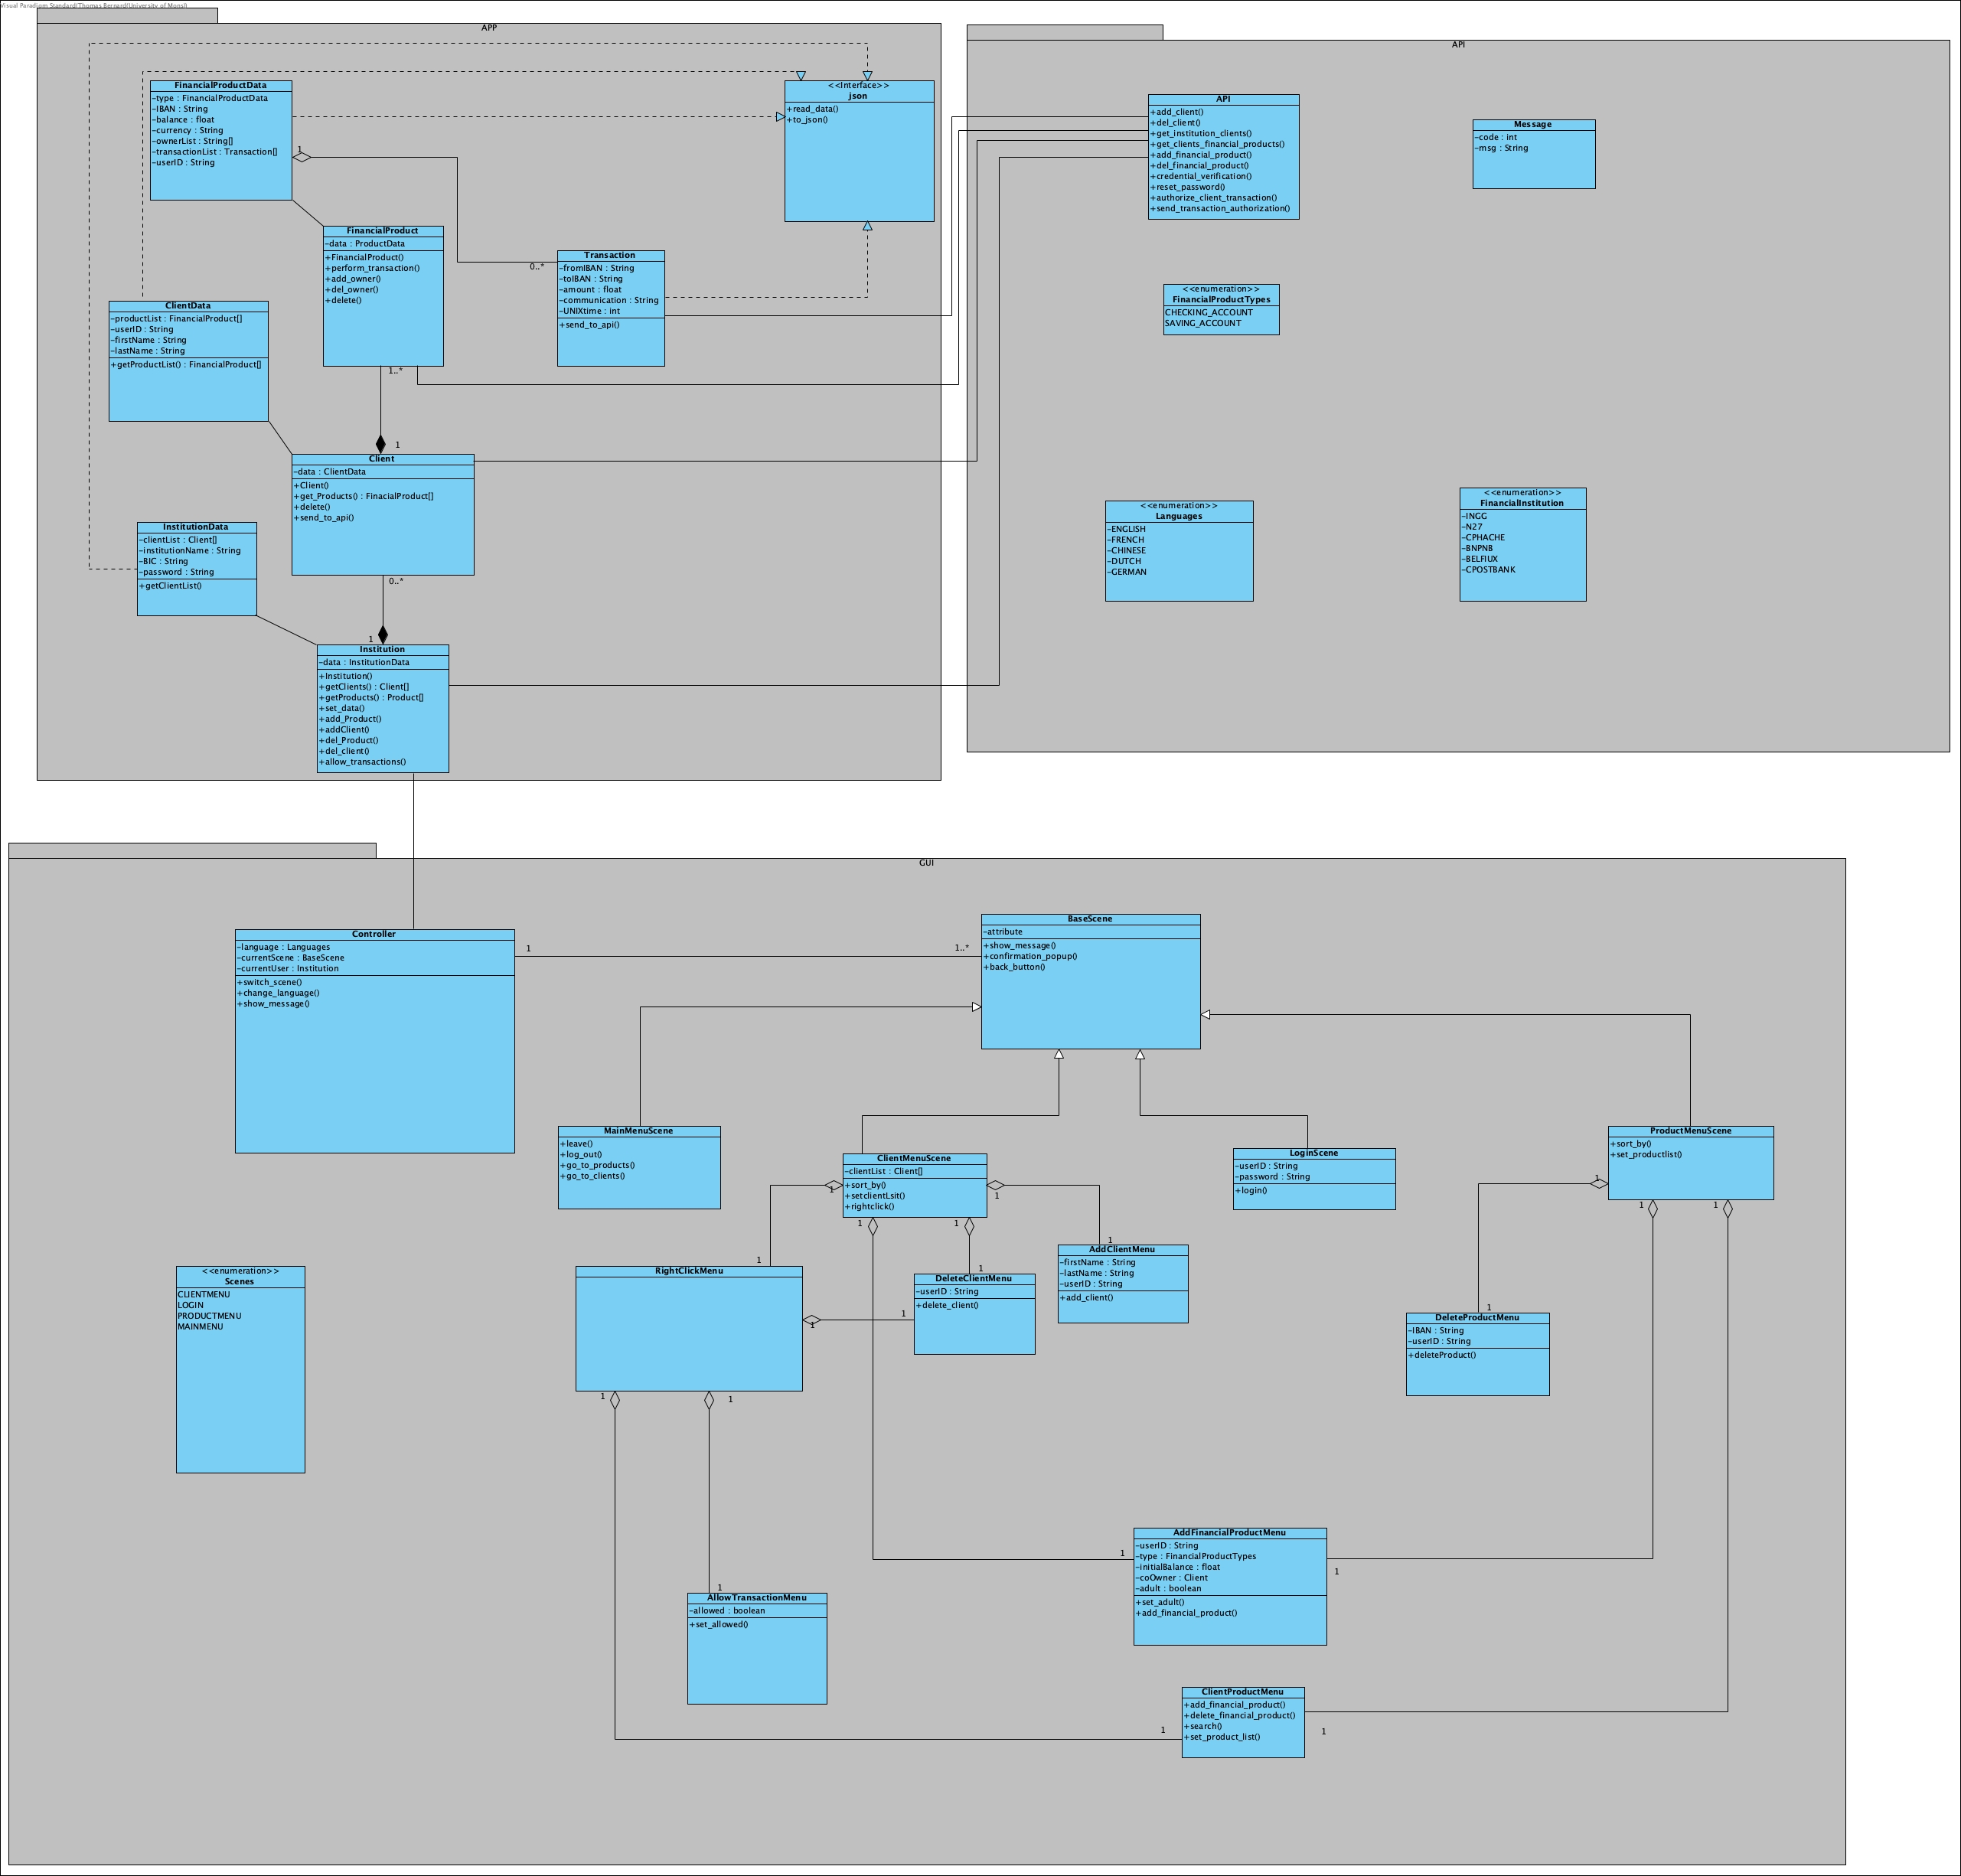
\includegraphics[scale=0.15]{ressources/photos_diagrammes/app2/classes2.jpg}
		\caption{Diagramme de classe de l'application 2}
\end{figure}
Les classes de l'application 2 ont également été divisées en 3 packages afin de garder une bonne organisation générale des classes.
Il y a donc un package APP qui contient la partie logique de l'application comme la représentation des objets, un package GUI contenant toutes les classes de l'interface graphique et un package API contenant toutes les classes permettant la communication avec le serveur et donc la base de données.\\

Pour la partie logique, chaque objet possède une classe Data permettant de créer un fichier JSON contenant les données de cet objet. Cela permettra de facilement envoyer des données au serveur via l'API.\\

La partie graphique de l'application est un ensemble de scène créées à partir d'une scène de base avec des méthodes globaux avec pour la plus part leurs menu qui eux contiennent des méthodes plus spécifique a une tache en particculier. Chaque scène est spécifique à une fenêtre de l'application et chaque menu est spécifique a une action pouvant être effectuer dans la scène.\\
La classe Controller du package GUI permettra de passer d'une scène à une autre. La navigation entre les scènes sera facilitée par l'enumeration Scenes contenant une énumération par scène. App possède également une référence vers un objet currenrtInstitution afin de pouvoir accéder aux données de l'institution courrante.\\

Les méthodes de l'API se résumeront globalement à l'envoi d'un message via HTTPS sur l'URI de l'API. Les paramètres sont passés directement dans l'URI ce qui posera des problèmes de sécurité lors de l'implémentation. (explication dans la partie API du rapport) \\
Pour passer des objets à l'API, nous utiliserons JSON ou YAML. Elle répond avec le même format. JSON ou YAML sont très simples à générer et à lire d'où le grand intérêt de leur utilisation. D'autres méthodes vont être nécessaires afin d'intéragir avec les fichiers JSON ou YAML.\\
\end{document}
